
\documentclass{article}
\usepackage{graphicx}
\usepackage{fullpage}
\usepackage{amsmath}
\usepackage{caption}
\usepackage{subcaption}
\usepackage{listings}
\usepackage{color}
\author{Jordan Milton\\ jksm1g10}
\title{Evolution of Complexity: Assignment 2}
\definecolor{javared}{rgb}{0.6,0,0} % for strings
\definecolor{javagreen}{rgb}{0.25,0.5,0.35} % comments
\definecolor{javapurple}{rgb}{0.5,0,0.35} % keywords
\definecolor{javadocblue}{rgb}{0.25,0.35,0.75} % javadoc
 
\lstset{language=Java,
basicstyle=\ttfamily,
keywordstyle=\color{javapurple}\bfseries,
stringstyle=\color{javared},
commentstyle=\color{javagreen},
morecomment=[s][\color{javadocblue}]{/**}{*/},
numbers=left,
numberstyle=\tiny\color{black},
stepnumber=1,
numbersep=10pt,
tabsize=4,
showspaces=false,
showstringspaces=false}

\begin{document}
\maketitle
\section{Introduction}
\subsection{Description}
One way in which the fitness of a genome in a Genetic Algorythm can be determined is by evaluating it against other genomes, which can provide several benefits over using an objective metric to measure performance. These benefits include:
\begin{description}
\item{\textbf{Providing a hittable target:}}
This is when evaluating the fitness of a genome by comparing it to another gives a better gradient for improvement over an objective metric. For instance, if a game playing machine was being evolved it would be more meaningful to compare it to other players of around the same ability than having them compete against a perfect player. This is because the latter makes it difficult to distinguish which genome is superior, where as in the former scenario this should become clear.
\item{\textbf{Providing a relevant target:}}
In some cases, in can be difficult to create a static test of fitness that makes the genome optimise all dimensions involved. To return to the game player example, it is possible to have the fitness be decided by the number of victorys against a predetermined set of other players. However it may be possible to beat these players without having optimised all dimensions. By having the opponent selected be another evolving genome the adaptive competition should focus the adaptation on aspects not yet optimised.
\item{\textbf{No defined end goal:}}
Another advantage of coevolution is that as the target moves with the fitness of the genome, there is nearly always room for improvement. To stick with the game player idea, with a fixed set of opponents once the genome outperforms all opponents it no longer has a target. However, when competing against other improving genomes there is always the possibility of becoming a better player than the best player found so far. Once found, this player is the new target.
\end{description}

However, it is also true that coevolution can introduce problems that would otherwise not exist. The problems introduced have a close relation to the problems it purportedly solves. The first issue relates to scenarios where in the populations seperate enough so that they no longer provide a good gradient for learning. The second issue relates to how focussing can create genomes that focus on the wrong things. Thus a generalist is never developed. The last issue is due to the loss of a objective fitness, and so it is possible that players do not improve in any objective sense. The paper that has been reimplemented provides a description of these, and then describes a minimal substrate for demonstrating those issues\cite{watson2001}. This minimal substrate consists of multiple number games played by competing genomes. This has two significant advantages. The first is that by having the fitness be determined by simple number games the algorythm is reasonably simple to implement. The second main reason is that it allows the objective fitness of genomes to be easily observed, even though it isn't used in the algorythm itself. This is often not the case in a real world application, which can make these problems difficult to spot.

\subsection{Experimental Setup}
In order to demonstrate the ideas discussed above, three different fitness functions need to be defined, with two different genome definitions. For the first game the genome will be defined as a binary string 100 bits long. The value of the genome will be determined as the number of 1s in the string. The fitness function is defined as:
\begin{equation}
fitness1(a, S) = \sum^{|S|}_{i=1}score1(a, S_i)
\end{equation}
\begin{equation}
score1(a, b) = \begin{cases}
1& \text{if $ a > b $}\\
0& \text{otherwise}
\end{cases}
\end{equation}

For the second game the genomes will have 10 dimensions opposed to the previous 1. However, the size of each dimension will be 10 bits. This keeps means that the sum of all dimensions still ranges from $ 0 - 100 $. The new fitness function will be defined as above, but only one dimension will be chosed for comparison. This will be decided by choosing the dimension in which the two genomes are most different. Below is a mathematical definition for the game for if it was in two dimensions instead of ten:
\begin{equation}
fitness2(a, S) = \sum^{|S|}_{i=1}score2(a, S_i)
\end{equation}
\begin{equation}
score2(a, b) = \begin{cases}
score1(a_x, b_x)& \text{if $ |a_x - b_x| > |a_y - b_y| $}\\
score1(a_y, b_y)& \text{otherwise}
\end{cases}
\end{equation}

For the last game, the only change is in the fitness function. Instead of picking the dimension the two genomes differ most, instead the dimension where they differ least is used for comparison. Below is the mathematical definition of the game in two dimensions instead of ten:
\begin{equation}
fitness3(a, S) = \sum^{|S|}_{i=1}score3(a, S_i)
\end{equation}
\begin{equation}
score3(a, b) = \begin{cases}
score1(a_x, b_x)& \text{if $ |a_x - b_x| < |a_y - b_y| $}\\
score1(a_y, b_y)& \text{otherwise}
\end{cases}
\end{equation}

The genetic algorythm will use a generational approach, and fitness proportionate selection will be used for choosing parents. For simplicity, the only variational operator will be mutation. For any test run with two populations, the sample to test against will be taken entirely from the other population. A table of all parameters is given below, assume these values are used unless otherwise stated.
\begin{table}[h]
\centering

\begin{tabular}{|c|c|}
\hline
\textbf{Variable} & \textbf{Value} \\ \hline\hline
Mutation Rate & 0.005 \\ \hline
Population Size & 25 \\ \hline
Sample Size & 15 \\ \hline
Number of Generations & 600 \\ \hline
Number of populations & 2 \\ \hline
\end{tabular}
\end{table}
\section{Reimplemented results}

This section goes through the experiments from the original paper alongside the results from the reimplementation. 

\begin{figure}
\centering
\begin{subfigure}{.5\textwidth}
  \centering
  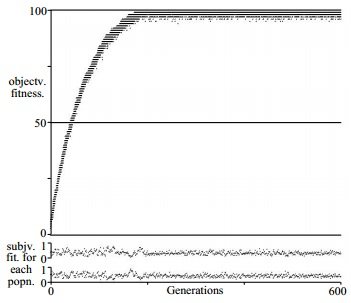
\includegraphics[width=.8\linewidth]{Screencaps/OneDimensionOrig}
  \caption{Original}
  \label{fig:eq1orig}
\end{subfigure}%
\begin{subfigure}{.5\textwidth}
  \centering
  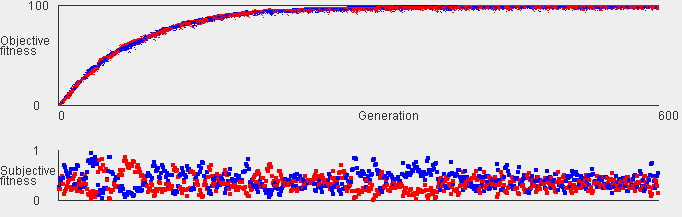
\includegraphics[width=\linewidth]{Screencaps/OneDimensionReimp}
  \caption{Reimplementation}
  \label{fig:eq1reimp}
\end{subfigure}
\caption{Coevolution using the first game}
\label{fig:eq1}
\end{figure}

Figure \ref{fig:eq1} shows the results from running the GA using the first fitness function. Red and blue in the reimplementation represent the two different populations. While this does reach the optimum state (objective fitness equals 100), the subjective fitness graph looks no different by generation 600 than it does at generation 300. What this shows is that the seperation of objective fitness from subjective fitness can make it difficult to know how well a coevolved population is progressing.

\begin{figure}
\centering
\begin{subfigure}{.5\textwidth}
  \centering
  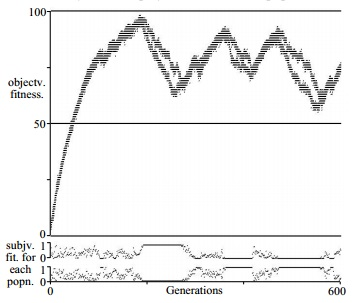
\includegraphics[width=.8\linewidth]{Screencaps/GradientLossOrig}
  \caption{Original}
  \label{fig:eq1S1orig}
\end{subfigure}%
\begin{subfigure}{.5\textwidth}
  \centering
  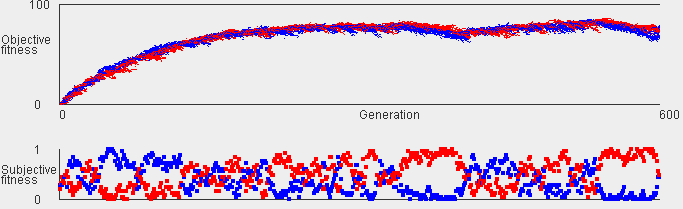
\includegraphics[width=\linewidth]{Screencaps/GradientLossReimp}
  \caption{Reimplementation}
  \label{fig:eq1S1reimp}
\end{subfigure}
\caption{Coevolution using the first game and sample size 1}
\label{fig:eq1S1}
\end{figure}

Next, the algorythm is run again. However this time the sample size is set to 1, so that each player plays against one genome from the other population. The result is shown in figure \ref{fig:eq1S1}. In both the original and the reimplemented result you can see that the algorythm now behaves completely differently. Looking at the subjective fitness, it can be seen that there are large peroids where the average fitness for either population is either 1 or 0. This means that genomes can't be differentiated and any selective pressure is lost. This leads to the ocassional phenomenon where the populations actually decrease in objective fitness, as without a selective pressure they drift until they reconnect with the other population. This effect is more obvious in the original but is still visible in the reimplementation.

\begin{figure}
\centering
\begin{subfigure}{.5\textwidth}
  \centering
  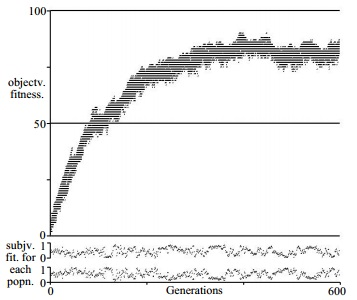
\includegraphics[width=.8\linewidth]{Screencaps/FocussingOrig}
  \caption{Original}
  \label{fig:eq2orig}
\end{subfigure}%
\begin{subfigure}{.5\textwidth}
  \centering
  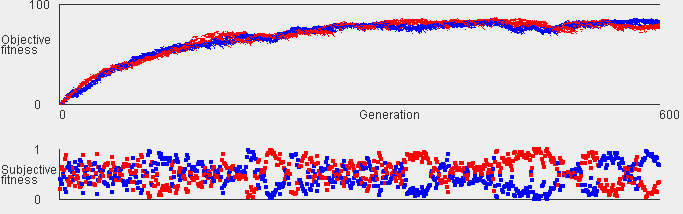
\includegraphics[width=\linewidth]{Screencaps/FocussingReimp}
  \caption{Reimplementation}
  \label{fig:eq2reimp}
\end{subfigure}
\caption{Coevolution using the second game}
\label{fig:eq2}
\end{figure}

The next test involves the second game and fitness function. The results of running this game can be seen in figure \ref{fig:eq2}. For the purpose of showing output, the objective fitness is the sum of all dimensions. This looks very similar to figure \ref{fig:eq1}, however unlike that experiment it fails to reach the optimal point at 100. While the selection pressure does seem to be changing what dimension is important, all other dimensions drift towards the mutation bias as described in the previous paper\cite{watson2001}. This means that it never produces a generalist.

\begin{figure}
\centering
\begin{subfigure}{.5\textwidth}
  \centering
  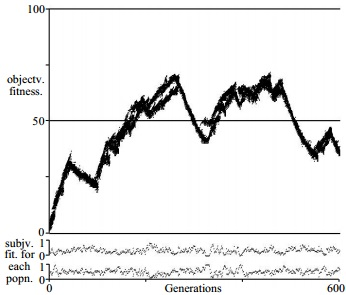
\includegraphics[width=.8\linewidth]{Screencaps/RelativismOrig}
  \caption{Original}
  \label{fig:eq3orig}
\end{subfigure}%
\begin{subfigure}{.5\textwidth}
  \centering
  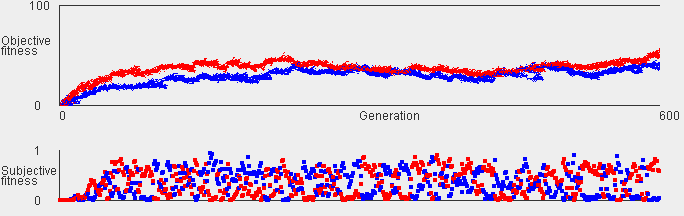
\includegraphics[width=\linewidth]{Screencaps/RelativismReimp}
  \caption{Reimplementation}
  \label{fig:eq3reimp}
\end{subfigure}
\caption{Coevolution using the third game}
\label{fig:eq3}
\end{figure}

The last experiment uses the third game. This test demonstrates the concept of relatavism where the selection pressure provided by coevolution fails to drive the population towards an objectively better genome. The results can be seen in figure \ref{fig:eq3}. Two big differences from figure \ref{fig:eq1} are immediately visible. The first is that neither population ever approaches the objective optimal point, and indeed sometimes actively moves away from it. The second is that the populations occassionally clearly split objectively, however not subjectively. The reason for this can be seen by inspecting the fitness function. Due to the nature of the function, it can occassionally be beneficial to reduce the value of a dimension. This can be either to increase the gap between a low scoring dimension and the genomes opponents, or to reduce a high scoring dimension to make it more relevant. This can occassionally lead to the objective fitness being driven down. The split in populations occurs because it is possible to win frequently with many very low scoring dimensions, indeed it is sometimes easier to do so.

\section{Extension}

\subsection{Hypothesis}
While evaluating the results of the second game, where the dimension of a genome being optimised changes causing other dimensions to drift back to the bias, it seemed like it might have the makings of being a building block problem\cite{watson2007, forrest1993}. The hypothesis then is that performing crossover in a population playing the second game will overcome the focussing problem.

The basis for this hypothesis is that while each high scoring genome has only necessitated optimising one dimension, it seems likely that different high scoring genomes will have scored well based on different dimensions. In that case, performing crossover should create a more generalist candidate. Over time this will hopefully lead to candidates that excell in all dimensions.

While this might initially seem like an attempt at a specific solution to this one game, the game is designed to be a simple example of a problem that exists in multiple real world applications. If making this change can create more generalists in this example, it is possible that a similar course of action could improve other systems that also suffer from focussing.

In order to carry out this test it is necessary to make a change to how children are created in the second game. Before mutation occurs, it will be necessary to take two genomes and perform crossover. The output of the crossover will be mutated and used as the child to be put in the next generation. The next question is then in what way will crossover be implemented. As the idea is to hopefully combine good dimensions from different individuals, fixed point crossover will be used. For simplicity, which parent a dimension is taken from for the child will be alternated. So parent one will pass on dimensions one, three, five, seven and nine. 

\subsection{Results}

The result of the hypothesis test is that crossover made no difference at all. As can be seen in figure \ref{fig:extend}, the output of the populations when performing crossover is almost identical to that of the populations without crossover (figure \ref{fig:eq2reimp}). No change is seen either in the objective or subjective fitness.
\begin{figure}
  \centering
  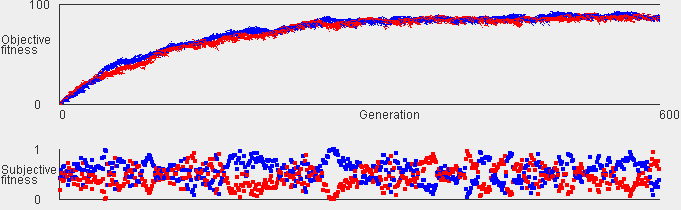
\includegraphics[width=.6\linewidth]{Screencaps/crossover}
  \caption{Game two with crossover}
  \label{fig:extend}
\end{figure}

This initially caused some confusion. While it wasn't necessarily expected to remove the problem completely, some movement was expected. It was suspected after a while that the problem was to do with a lack of diversity in the populations, at least among the high scoring genomes. To test this, one population was selected. For every genome in the population, if it won more than a quarter of the games played the highest scoring dimension was recorded. Those who scored less are ignored as they are deemed unlikely to reproduce. From that, it was determined which dimension was most favored by high scorers that generation, and what proportion of high scorers had optimised that dimension. This was recorded for every generation, along with a count of all individuals that scored above the cap. This was graphed accross all generations, and can be seen in figure \ref{fig:diversity}. The blue line represents the total of players above the cap, and the red line the number that optimised the same dimension. The y axis ranges from 0 at the bottom to the total population count, and the x axis ranges from 0 to 600. 

\begin{figure}
  \centering
  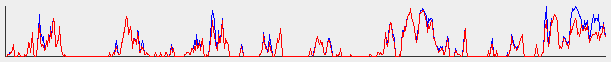
\includegraphics[width=.6\linewidth]{Screencaps/diversity}
  \caption{Test of Diversity}
  \label{fig:diversity}
\end{figure}

As can be seen in figure \ref{fig:diversity}, there is very little diversity amongst individuals likely to reproduce. Most of the time, the number of individuals above the cap and the number that have optimised the same dimension are the same. This means that crossover will have no effect as they have all built the same blocks, and nothing is gained during crossover. However, when observing the value for whether the best dimension has also been maximised it turns out that this is usually the case. As can be seen in figure \ref{fig:optomised}. The axis of the graph are the same as the previous one, and the blue line again represents players above the cap. However, the red line in this case represents those players who score 10 in their best dimension.
\begin{figure}
  \centering
  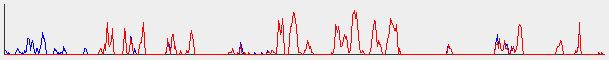
\includegraphics[width=.6\linewidth]{Screencaps/optomised}
  \caption{Number of players with a maximised dimension}
  \label{fig:optomised}
\end{figure}
In conclusion, the hypothesis was incorrect. Adding crossover to the reproduction of new individuals does not alleviate the problem of focussing in coevolution. Based on the results, however, it would be interesting to redo the experiment with some diversity maintenance. As has been shown, the players do build the whole of their block. The issue is with diversity, and that there is nothing to be gained in crossover in this set up. If diversity maintenance were introduced, that could make crossover worthwhile and alleviate the focussing problem.

\bibliographystyle{plain}
\bibliography{report}
\appendix
\section{GameRunner}
\lstinputlisting[language=Java, breaklines=true]{../Code/src/controller/GameRunner.java}
\section{GreatestGapScorer}
\lstinputlisting[language=Java, breaklines=true]{../Code/src/controller/GreatestGapScorer.java}
\section{OneDimScorer}
\lstinputlisting[language=Java, breaklines=true]{../Code/src/controller/OneDimScorer.java}
\section{SmallestGapScorer}
\lstinputlisting[language=Java, breaklines=true]{../Code/src/controller/SmallestGapScorer.java}
\section{DefaultMember}
\lstinputlisting[language=Java, breaklines=true]{../Code/src/model/DefaultMember.java}
\section{MemberInterface}
\lstinputlisting[language=Java, breaklines=true]{../Code/src/model/MemberInterface.java}
\section{Population}
\lstinputlisting[language=Java, breaklines=true]{../Code/src/model/Population.java}
\section{ScoringInterface}
\lstinputlisting[language=Java, breaklines=true]{../Code/src/model/ScoringInterface.java}
\section{MultiDimView}
\lstinputlisting[language=Java, breaklines=true]{../Code/src/view/MultiDimView.java}
\section{OneDimGraphPanel}
\lstinputlisting[language=Java, breaklines=true]{../Code/src/view/OneDimGraphPanel.java}
\end{document}